%%%%%%%%%%%%%%%%%%%%%%%%%%%%%%%%%
% Iterations                    %
%%%%%%%%%%%%%%%%%%%%%%%%%%%%%%%%%

\section{ITERATIONS}
\label{sec:iterations}

\noindent
The development of the synthesizer parameter estimation system followed a systematic iteration-based process guided by the Design Science Research framework introduced in Section~\ref{sec:methodology}. Three successive iterations — V1, V2, and V3 — were conducted, each corresponding to a complete DSR cycle in which a version of the artifact was designed, implemented, and evaluated, with empirical findings feeding directly into the design of the subsequent iteration. Each iteration introduces a distinct set of architectural or data-regime improvements motivated by the limitations uncovered in the preceding cycle.

% ─────────────────────────────────────────────────────────
\subsection{Data Generation Pipeline}

The data generation pipeline transforms raw synthesizer parameter configurations into a normalized, split dataset ready for model training. It consists of six sequential steps, illustrated in Figure~\ref{fig:pipeline}. Each step is designed to be checkpoint-aware and resumable, as the full pipeline involves several hours of audio rendering and processing.

\begin{figure}[H]
\centering
\begin{tikzpicture}[
  node distance=0.55cm and 0.9cm,
  box/.style={rectangle, rounded corners=6pt, draw=gray!60, fill=blue!7,
              text width=3.0cm, align=center, minimum height=1.3cm, font=\small},
  arrow/.style={-{Stealth[length=3.5mm]}, thick, gray!60}
]

% Row 1
\node[box] (s1) {\textbf{Step 1}\\[3pt]Parameter\\Extraction};
\node[box, right=of s1] (s2) {\textbf{Step 2}\\[3pt]Preset\\Generation};
\node[box, right=of s2] (s3) {\textbf{Step 3}\\[3pt]Audio\\Rendering};

% Row 2 (right to left below row 1)
\node[box, below=of s3] (s4) {\textbf{Step 4}\\[3pt]Silence\\Filtering};
\node[box, left=of s4]  (s5) {\textbf{Step 5}\\[3pt]Mel Spectrogram\\Extraction};
\node[box, left=of s5]  (s6) {\textbf{Step 6}\\[3pt]Dataset Split\\\& Normalization};

% Arrows
\draw[arrow] (s1) -- (s2);
\draw[arrow] (s2) -- (s3);
\draw[arrow] (s3) -- (s4);
\draw[arrow] (s4) -- (s5);
\draw[arrow] (s5) -- (s6);

% Corner connector
\draw[arrow] (s3.south) -- (s4.north);

\end{tikzpicture}
\vspace{0.3cm}
\caption{The six-step data generation pipeline, from parameter extraction to normalized dataset splits.}
\label{fig:pipeline}
\end{figure}

% ─────────────────────────────────────────────────────────
\subsubsection{Step 1: Parameter Extraction from Vital}

All 16 target parameters are enumerated programmatically from Vital via the Pedalboard Python library, which exposes the synthesizer's internal parameter table. For each parameter, the extraction records its name, internal plugin index, valid range $[x^{\min}_k,\, x^{\max}_k]$, and discretization information where applicable. While all parameters are exposed with continuous-looking ranges, Vital internally quantizes seven of them to a finite set of valid discrete values. Although these parameters may appear continuous from outside the synthesizer, Vital's internal implementation restricts them to specific grids:

\begin{itemize}
    \item \textbf{Envelope times} (\texttt{env1\_attack}, \texttt{env1\_decay}, \texttt{env2\_attack}, \texttt{env2\_decay}): Despite being specified in seconds over a wide range, all four envelope times are mapped to 1{,}001 discrete steps on a logarithmic time grid. This quantization reflects the resolution of Vital's internal envelope generator, meaning that many nominally distinct floating-point time values collapse to the same rendered behaviour.

    \item \textbf{Filter cutoff} (\texttt{filter1\_cutoff}): Expressed in semitones over a broad pitch range, the filter cutoff is internally quantized to 1{,}001 discrete frequency values. Although the parameter appears continuous, Vital's filter implementation operates on a fixed frequency grid of that resolution.

    \item \textbf{Unison voice count} (\texttt{osc1\_unison\_voices}): Controls how many detuned copies of oscillator 1 are layered to produce a thicker sound. This parameter is inherently discrete, as a fractional number of voices has no physical meaning within the synthesizer engine.

    \item \textbf{Oscillator 2 transpose} (\texttt{osc2\_transpose}): Sets the pitch offset of oscillator 2 relative to the played note. This parameter is inherently discrete by musical convention, taking only integer semitone values.
\end{itemize}

The extracted ranges and discrete value tables are stored as JavaScript Object Notation (JSON) reference files and used throughout the pipeline. Table~\ref{tab:parameters} lists all 16 parameters in their prediction order, along with their discrete status and a brief description.

\begin{table}[H]
\centering
\renewcommand{\arraystretch}{1.35}
\begin{tabular}{clcp{6.5cm}}
\hline
\textbf{\#} & \textbf{Parameter} & \textbf{Discrete} & \textbf{Description} \\
\hline
0  & \texttt{osc1\_wave\_frame}    & ---  & Wavetable position of oscillator 1, controlling the spectral shape of its output waveform. \\
1  & \texttt{osc1\_level}          & ---  & Output amplitude of oscillator 1. \\
2  & \texttt{osc1\_unison\_voices} & Yes  & Number of detuned voices layered by oscillator 1 to produce a thicker sound. \\
3  & \texttt{osc1\_unison\_detune} & ---  & Pitch spread between the unison voices of oscillator 1. \\
4  & \texttt{osc2\_wave\_frame}    & ---  & Wavetable position of oscillator 2, controlling its spectral character. \\
5  & \texttt{osc2\_level}          & ---  & Output amplitude of oscillator 2. \\
6  & \texttt{osc2\_transpose}      & Yes  & Pitch offset of oscillator 2 relative to the played note, in integer semitone steps. \\
7  & \texttt{env1\_attack}         & Yes  & Attack time of the amplitude envelope (Envelope 1). \\
8  & \texttt{env1\_decay}          & Yes  & Decay time of the amplitude envelope (Envelope 1). \\
9  & \texttt{env2\_attack}         & Yes  & Attack time of the filter envelope (Envelope 2). \\
10 & \texttt{env2\_decay}          & Yes  & Decay time of the filter envelope (Envelope 2). \\
11 & \texttt{filter1\_cutoff}      & Yes  & Low-pass filter cutoff frequency, specified in semitones. \\
12 & \texttt{filter1\_resonance}   & ---  & Resonance (Q factor) of the low-pass filter. \\
13 & \texttt{sample\_level}        & ---  & Output amplitude of the noise/sample oscillator. \\
14 & \texttt{mod1\_amount}         & ---  & Depth of filter envelope modulation applied to the filter cutoff. \\
15 & \texttt{reverb\_mix}          & ---  & Wet/dry mix of the global reverb effect. \\
\hline
\end{tabular}
\vspace{0.3cm}
\caption{All 16 synthesizer parameters extracted from Vital, listed in prediction order (index 0--15). \textit{Discrete} indicates parameters that Vital internally quantizes to a finite set of valid values despite appearing continuous from outside the synthesizer. Sustain and release are excluded as both are unobservable in a fixed 4-second render with no note-off event.}
\label{tab:parameters}
\end{table}

% ─────────────────────────────────────────────────────────
\subsubsection{Step 2: Timbre-Constrained Preset Generation}

A naive uniform sampling of the 16-dimensional parameter space produces predominantly silent, extremely bright, or otherwise pathological sounds of little musical relevance. To ensure that the dataset covers a representative range of practically meaningful sounds, a \textit{timbre-constrained} generation strategy is employed. Five timbre categories are defined, each associated with a set of parameter sub-ranges that constrain the sampling to musically coherent regions of the parameter space. The categories and their MIDI pitch ranges are summarized in Table~\ref{tab:timbre_categories}.

\begin{table}[H]
\centering
\renewcommand{\arraystretch}{1.3}
\begin{tabular}{lcccp{4.5cm}}
\hline
\textbf{Timbre} & \textbf{Min MIDI} & \textbf{Max MIDI} & \textbf{Presets} & \textbf{Sound characteristics} \\
\hline
bass   & C0 (12) & C3 (48) & 6{,}000  & Low register; slow amplitude envelope; sub-bass and bass tones. \\
lead   & C3 (48) & C6 (84) & 6{,}000  & Mid-to-high register; bright, cutting timbre suitable for melodic lines. \\
pad    & C2 (36) & C5 (72) & 6{,}000  & Sustained chordal texture; slow attack to emphasise the hold phase. \\
percs  & C1 (24) & C6 (84) & 6{,}000  & Very short attack; noise/sample oscillator prominent; percussive hits. \\
random & C0 (12) & C6 (84) & 20{,}000 & Unconstrained sampling across the full parameter and pitch range. \\
\hline
\textbf{Total} & & & \textbf{44{,}000} & \\
\hline
\end{tabular}
\vspace{0.3cm}
\caption{Timbre categories used for preset generation, with their MIDI pitch ranges, preset counts, and target sound characteristics.}
\label{tab:timbre_categories}
\end{table}

\noindent Each timbre category is governed by a dedicated JSON range file that narrows the sampling bounds of the 16 parameters to a musically coherent region. Within those bounds, parameter values are drawn at random, so the resulting sounds vary widely in character while still belonging recognisably to the target category. The \texttt{percs} category, for instance, caps the amplitude attack at 10\,ms, constrains the decay to a moderate range, and keeps the noise/sample oscillator level high — guaranteeing that every randomly drawn preset produces a percussive hit regardless of the exact values selected for the remaining parameters. Once generated, each preset is appended as a record to a per-timbre JSON Lines (JSONL) file. The generation loop is checkpoint-aware: a hash of each parameter vector is checked against previously written entries, so an interrupted run can be safely resumed from where it left off without introducing duplicates.

% ─────────────────────────────────────────────────────────
\subsubsection{Step 3: Audio Rendering}

Each preset is rendered to a 44.1 kHz mono WAV file via Pedalboard, which loads Vital as a VST3 plugin, sets all 16 parameters programmatically, and triggers a MIDI note-on event without a corresponding note-off. The clip duration is fixed at 4 seconds. The absence of a note-off event means that the release stage of the amplitude envelope is never triggered, which is why release is excluded from the 16 studied parameters. The sustain stage is similarly excluded, as the envelope decay is set long enough relative to the 4-second clip to produce effectively sustained sounds without requiring an explicit sustain parameter.

\par \vspace{0.3cm}
In V1 and V2, each preset is rendered at a single MIDI pitch sampled uniformly from the timbre's valid range. In V3, each preset is re-rendered at up to three fixed MIDI pitches per timbre (Table~\ref{tab:v3_midi}), selected to cover the low, mid, and high registers of the timbre's range. A hash keyed on the (sorted preset parameters, MIDI note) pair is used to detect already-rendered combinations: if the V1/V2 random note coincides with one of the three fixed notes, that render already exists and is skipped, and only the remaining two fixed notes are rendered; if the V1/V2 note differs from all three fixed notes, all three are rendered. Each preset therefore ends up with either three clips (if the V1 note matched one fixed note) or four clips (if it matched none), with four being the typical outcome since the random V1 note rarely coincides with the fixed schedule. The same hash mechanism enables safe resumption of interrupted runs. Rendered audio paths and ground-truth parameters are written to a combined JSONL file with one record per clip.

% ─────────────────────────────────────────────────────────
\subsubsection{Step 4: Silence Filtering}

Certain extreme parameter combinations cause Vital to produce no audible output — for example, when both oscillators are muted and the sample level is zero. These silent clips are detected and removed using a hybrid energy-based rule applied to each rendered WAV file.

\par \vspace{0.3cm}
\noindent A straightforward approach would compute the mean energy of the full 4-second clip and discard anything below a fixed threshold. This fails for percussive and transient-heavy sounds: a stab, a drum hit, or a pluck concentrates nearly all of its energy in the first 10--100~ms of the clip, leaving the remaining 3.9+ seconds close to silence. The clip-level mean energy for such sounds can fall well below any reasonable threshold even when the sound itself is perfectly audible and musically useful. The detector must therefore distinguish between a clip that is uniformly quiet throughout and one that is quiet on average but contains a brief burst of high energy. The hybrid rule introduced below addresses this by combining an activity-based criterion, which checks what fraction of the clip has meaningful energy, with a peak-based criterion, which checks whether any moment in the clip reaches a minimum loudness level.

\par \vspace{0.3cm}
The audio signal $x(n)$ is divided into short frames of length $L$ with hop $H$. The Root Mean Square (RMS) energy of the $i$-th frame is computed as:

\begin{equation}
E_i = \sqrt{\frac{1}{L} \sum_{n=0}^{L-1} x^2(iH + n)}
\label{eq:rms}
\end{equation}

\noindent and converted to decibels:

\begin{equation}
E_i^{\text{dB}} = 20 \cdot \log_{10}(E_i + \epsilon)
\label{eq:rms_db}
\end{equation}

\noindent where $\epsilon$ is a small floor value to avoid $\log(0)$. Two detection rules are then applied:

\begin{equation}
R = \frac{1}{N_f} \sum_{i=1}^{N_f} \mathbf{1}\!\left[E_i^{\text{dB}} > \theta_{\text{rms}}\right]
\label{eq:active_ratio}
\end{equation}

\begin{equation}
P^{\text{dB}} = \max\!\left(\max_{i}\, E_i^{\text{dB}},\;\; 20 \cdot \log_{10}\!\left(\max_{n}\,|x(n)|\right)\right)
\label{eq:peak_db}
\end{equation}

\noindent where $R$ is the \textit{active ratio} — the fraction of frames exceeding the RMS threshold $\theta_{\text{rms}}$ — and $P^{\text{dB}}$ is the peak energy measure, defined as the maximum of the highest frame RMS in decibels and the peak sample amplitude in decibels. Taking the maximum of both is equivalent to flagging a clip as non-silent if either measure exceeds the threshold, which is how the detector is implemented. A clip is retained if either condition is satisfied:

\begin{equation}
\text{keep} \;\Leftrightarrow\; \left(R > \rho_{\min}\right) \;\vee\; \left(P^{\text{dB}} > \theta_{\text{peak}}\right)
\label{eq:keep_rule}
\end{equation}

\noindent The logical OR ensures that transient-heavy sounds such as percussions — which concentrate energy in a small number of frames and would fail the active ratio rule alone — are not incorrectly discarded. The per-timbre thresholds are given in Table~\ref{tab:silence_thresholds}.

\begin{table}[H]
\centering
\renewcommand{\arraystretch}{1.3}
\begin{tabular}{lccc}
\hline
\textbf{Timbre} & $\boldsymbol{\theta_{\text{rms}}}$ \textbf{(dB)} & $\boldsymbol{\rho_{\min}}$ & $\boldsymbol{\theta_{\text{peak}}}$ \textbf{(dB)} \\
\hline
bass   & $-50.0$ & $0.020$ & $-28.0$ \\
lead   & $-50.0$ & $0.020$ & $-28.0$ \\
pad    & $-55.0$ & $0.015$ & $-30.0$ \\
percs  & $-50.0$ & $0.002$ & $-30.0$ \\
random & $-50.0$ & $0.010$ & $-30.0$ \\
\hline
\end{tabular}
\vspace{0.3cm}
\caption{Per-timbre silence detection thresholds used in the hybrid RMS filtering step.}
\label{tab:silence_thresholds}
\end{table}

% ─────────────────────────────────────────────────────────
\subsubsection{Step 5: Mel Spectrogram Extraction}

Each surviving audio clip is converted to a mel spectrogram representation. Given the discrete-time audio signal $x(n)$ at sample rate $f_s = 44{,}100$ Hz, the Short-Time Fourier Transform (STFT) is first computed as:

\begin{equation}
X(t, f) = \sum_{n} x(n)\, w(n - tH)\, e^{-j2\pi fn/N}
\label{eq:stft}
\end{equation}

\noindent where $w$ is a Hann window of length $N$ (the FFT size), $H$ is the hop length, and $t$ indexes time frames. The power spectrogram is then obtained as:

\begin{equation}
P(t, f) = |X(t, f)|^2
\label{eq:power_spec}
\end{equation}

\noindent A bank of $M = 128$ triangular mel filters $\{H_m(f)\}_{m=1}^{M}$, spaced according to the mel scale between $f_{\min} = 20$ Hz and $f_{\max} = 12{,}000$ Hz, is applied to yield the mel spectrogram:

\begin{equation}
S(t, m) = 10 \cdot \log_{10}\!\left(\sum_{f} H_m(f)\, P(t, f) + \epsilon\right)
\label{eq:mel}
\end{equation}

\noindent This produces a $128 \times T$ matrix, where $T$ is the number of time frames.

\par \vspace{0.3cm}
\noindent \textbf{V1 --- Single-Scale.} A single mel spectrogram is extracted using the mid-scale FFT configuration (Table~\ref{tab:mel_scales}) and stored as a \texttt{.npy} file.

\par \vspace{0.3cm}
\noindent \textbf{V2 --- Multi-Scale.} Three mel spectrograms are extracted per clip at fine, mid, and coarse resolutions. As the FFT window size increases, spectral resolution improves at the cost of temporal resolution, and vice versa. Table~\ref{tab:mel_scales} lists the parameters of each scale and the type of information each captures.

\begin{table}[H]
\centering
\renewcommand{\arraystretch}{1.3}
\begin{tabular}{lcccp{4.5cm}}
\hline
\textbf{Scale} & \textbf{n\_fft} & \textbf{Hop} & \textbf{Raw Frames ($T$)} & \textbf{Captures} \\
\hline
Fine   & 512     & 128     & $\approx$1{,}378 & Attack transients, onset details \\
Mid    & 2{,}048 & 512     & $\approx$345     & Timbral balance, envelope shape  \\
Coarse & 8{,}192 & 2{,}048 & $\approx$87      & Harmonic structure, pitch content \\
\hline
\multicolumn{5}{l}{\small All scales: 128 mel bins, $f_{\min}=20$ Hz, $f_{\max}=12{,}000$ Hz, $f_s=44{,}100$ Hz.}\\
\multicolumn{5}{l}{\small All inputs padded or truncated to 224 time frames for ConvNeXt/AST.}\\
\hline
\end{tabular}
\vspace{0.3cm}
\caption{Multi-scale mel spectrogram configurations used in V2 and V3.}
\label{tab:mel_scales}
\end{table}

Figure~\ref{fig:multiscale_mel_example} shows the three spectrograms computed from the same bass note (MIDI 36) rendered by Vital. At the fine scale, the rapid amplitude modulation caused by the unison voices is clearly visible along the time axis. At the mid scale, the overall envelope shape and timbral balance come into focus. At the coarse scale, the individual harmonics of the note resolve into distinct horizontal bands, making pitch-related information far more legible. Each scale therefore contributes information that the others cannot provide, which is the core motivation for stacking them.

\begin{figure}[H]
\centering
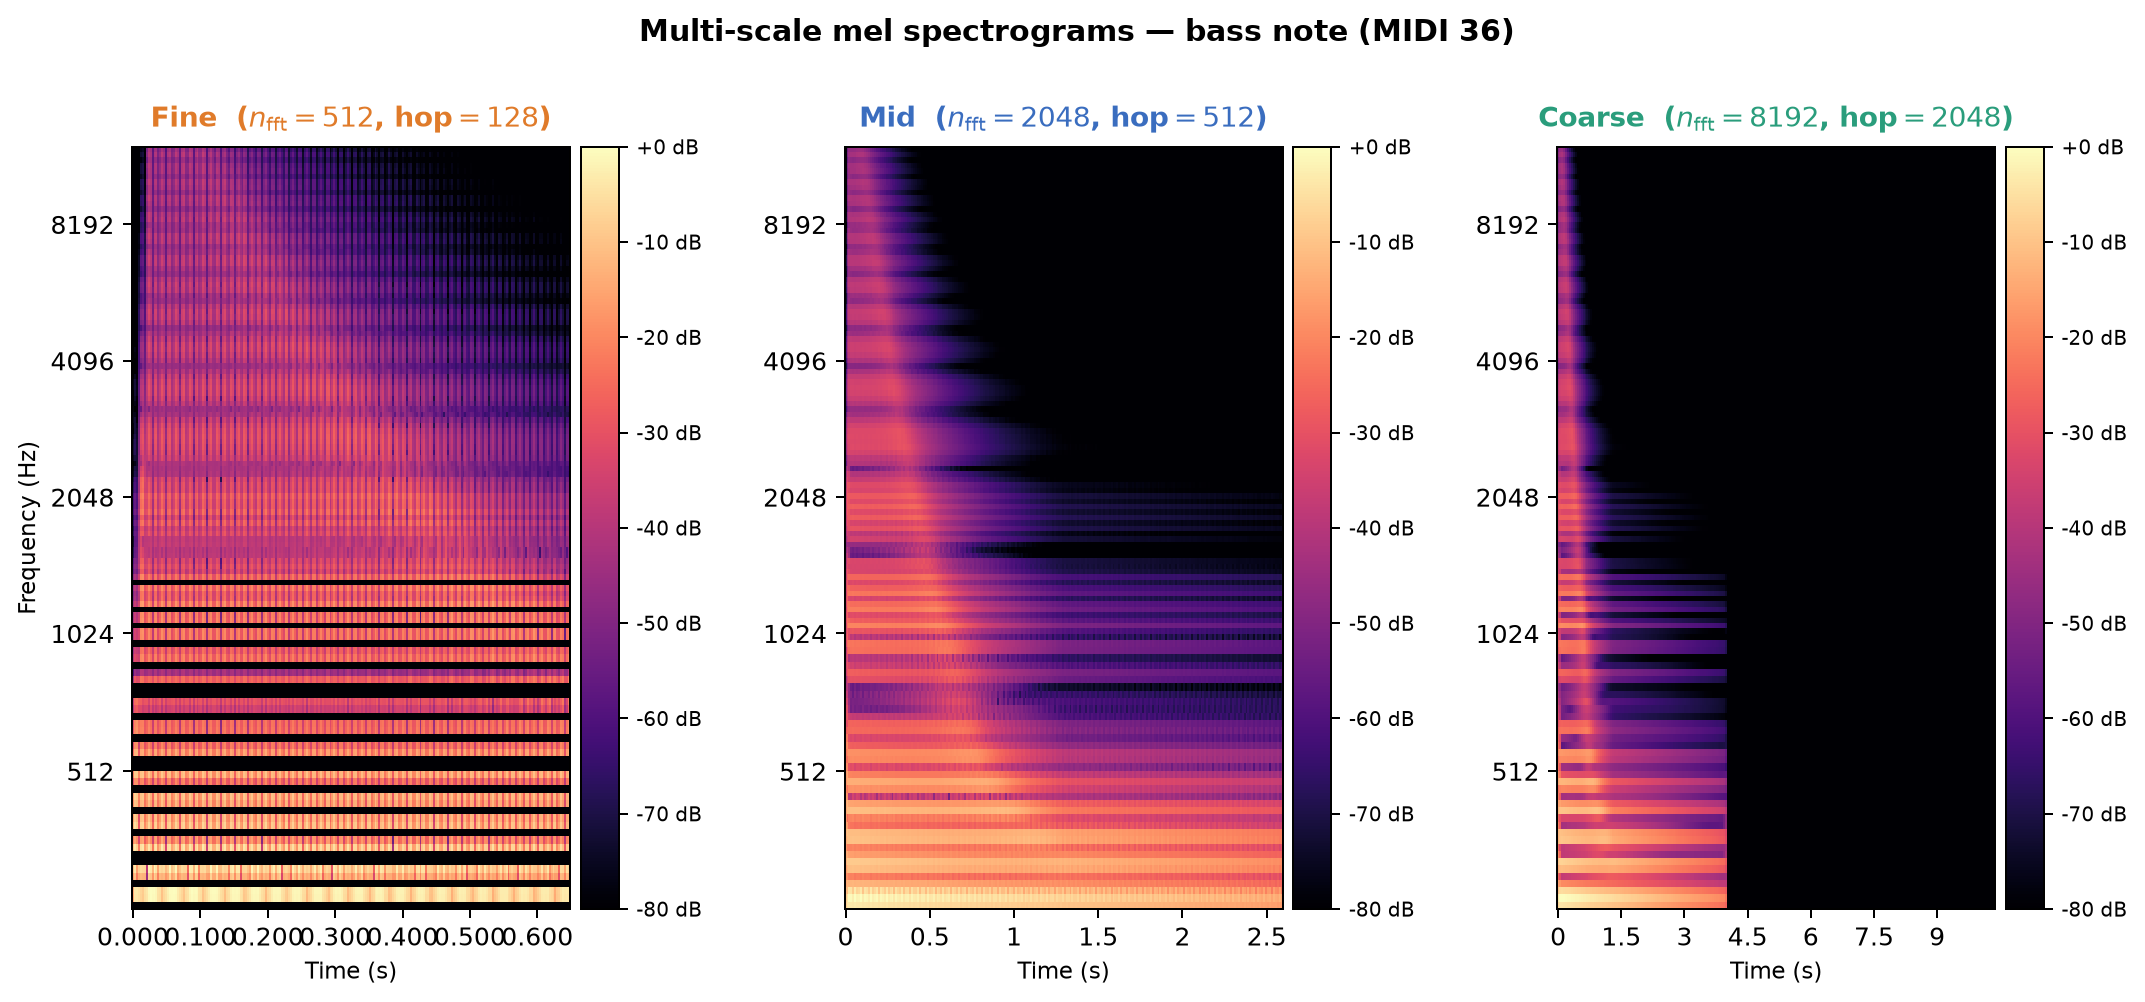
\includegraphics[width=\linewidth]{images/multiscale_mel_example.png}
\vspace{0.2cm}
\caption{Multi-scale mel spectrograms of a Vital bass note (MIDI 36) at fine ($n_{\text{fft}}=512$), mid ($n_{\text{fft}}=2{,}048$), and coarse ($n_{\text{fft}}=8{,}192$) resolutions. The fine scale resolves fast temporal events; the mid scale shows envelope shape and spectral balance; the coarse scale reveals the harmonic series structure. All three are padded or truncated to 224 time frames before stacking.}
\label{fig:multiscale_mel_example}
\end{figure}

\noindent The three spectrograms are stacked along the channel dimension to form a three-channel input tensor of shape $(3, 128, 224)$, as illustrated in Figure~\ref{fig:multiscale_stack}. This is directly compatible with the three-channel (RGB) first-layer weight initialization of ConvNeXt and ViT backbones.

\begin{figure}[H]
\centering
\begin{tikzpicture}[
  spec/.style={draw=gray!60, fill=blue!6, minimum width=3.8cm, minimum height=1.1cm,
               align=center, font=\small},
  label/.style={font=\small, align=center},
  arrow/.style={-{Stealth[length=4mm]}, thick, gray!50}
]

% Three spectrogram slabs
\node[spec, fill=orange!12] (fine)   at (0, 2.6) {Fine\\$n_{\text{fft}}=512$};
\node[spec, fill=blue!10]   (mid)    at (0, 1.3) {Mid\\$n_{\text{fft}}=2048$};
\node[spec, fill=teal!10]   (coarse) at (0, 0.0) {Coarse\\$n_{\text{fft}}=8192$};

\node[label] at (0, -0.7) {$128\times224$ each};

% Brace / arrow
\draw[arrow] (2.2, 1.3) -- (3.4, 1.3);

% Stacked tensor box
\draw[fill=gray!8, draw=gray!60, rounded corners=4pt]
  (3.5, 0.3) rectangle (5.5, 2.3);
\node[font=\small, align=center] at (4.5, 1.3)
  {$(3, 128, 224)$\\\small tensor};

% Channel labels inside
\draw[fill=orange!12, draw=gray!40] (3.6, 1.75) rectangle (5.4, 2.15);
\draw[fill=blue!10,   draw=gray!40] (3.6, 1.25) rectangle (5.4, 1.65);
\draw[fill=teal!10,   draw=gray!40] (3.6, 0.45) rectangle (5.4, 0.85);
\node[font=\tiny] at (4.5, 1.95) {ch 0: Fine};
\node[font=\tiny] at (4.5, 1.45) {ch 1: Mid};
\node[font=\tiny] at (4.5, 0.65) {ch 2: Coarse};

\end{tikzpicture}
\vspace{0.3cm}
\caption{Three mel spectrograms at fine, mid, and coarse resolutions stacked into a single three-channel input tensor of shape $(3, 128, 224)$.}
\label{fig:multiscale_stack}
\end{figure}

% ─────────────────────────────────────────────────────────
\subsubsection{Step 6: Dataset Splitting and Normalization}

\subsubsubsection{Stratified Split}

A purely random partition would not guarantee that each set reflects the full musical diversity of the dataset. By chance, all bass presets could land predominantly in the training set while the test set is dominated by pad or random presets, or an entire pitch register could be absent from validation entirely. Under such a split, the reported MAE would partly reflect a distribution mismatch rather than a genuine measure of model generalisation. The stratified split prevents this by treating the joint timbre-and-pitch-register label as a stratum and allocating samples from each stratum in the target 80\,/\,10\,/\,10 ratio independently, ensuring that every timbre category and every pitch register appears in proportional numbers across all three partitions. This guarantees that the evaluation sets are musically representative: the model is tested on the same joint distribution of sounds it was trained on, so MAE differences between configurations reflect differences in model quality rather than accidents of split composition.

Each sample is assigned a bucket key combining its timbre label and the octave of its MIDI note:

\begin{equation}
\text{bucket} = \left(\text{timbre},\; \left\lfloor \frac{\text{midi\_note}}{12} \right\rfloor\right)
\label{eq:bucket}
\end{equation}

\noindent Within each bucket, sample indices are deterministically shuffled using a seeded random number generator and then allocated in an 80\,/\,10\,/\,10 ratio to training, validation, and test sets in that order. A guard ensures that at least one sample from every non-empty bucket falls in the training partition, preventing pathologically small strata from being entirely consumed by the test allocation. Five independent splits are generated using seeds 42 through 46, producing five-fold cross-validation partitions for robust evaluation of the $\approx 42{,}520$-sample V1/V2 dataset. Reporting test MAE as mean $\pm$ standard deviation across the five folds controls for the variance introduced by any single arbitrary split.

\par \vspace{0.3cm}
In V3, sample-level splitting introduces a data leakage problem that does not exist in V1 or V2. Because each preset is rendered at three MIDI pitches, a sample-level split could assign two of a preset's renders to the training partition and the third to the test partition. As all three renders share the same parameter target $\mathbf{y}$, the model would have encountered those exact synthesis parameters during training, artificially deflating the reported test MAE. The V3 split therefore operates at the preset level: all renders of the same preset are treated as a single indivisible group, and entire groups are assigned to partitions rather than individual samples. The group key is computed as the MD5 hash of the 16 parameter values:

\begin{equation}
k(\theta) = \mathrm{MD5}\!\left(\theta_0,\, \theta_1,\, \ldots,\, \theta_{15}\right)
\label{eq:preset_key}
\end{equation}

\noindent This hash is deterministic and identical across all MIDI-note renders of the same preset without requiring a stored group identifier in the dataset. Figure~\ref{fig:preset_split} contrasts the two splitting strategies.

\begin{figure}[H]
\centering
\resizebox{\linewidth}{!}{%
\begin{tikzpicture}[
  font=\small,
  cbox/.style={rectangle, rounded corners=3pt, draw=gray!55,
               minimum height=0.72cm, text width=1.45cm, align=center, font=\scriptsize},
  pbox/.style={rectangle, rounded corners=4pt, draw=gray!65, fill=orange!10,
               minimum height=0.88cm, text width=1.9cm, align=center},
  arr/.style={-{Stealth[length=2.5mm]}, thick, gray!55},
]

%% LEFT PANEL (incorrect)
\node[font=\small\bfseries, text=red!60]  at (-3.4, 5.4)  {Sample-level split};
\node[font=\scriptsize, text=gray!65]     at (-3.4, 5.05) {(incorrect for V3)};

\node[pbox] (PL) at (-3.4, 4.3)
  {Preset $\theta_1$\\[-2pt]\scriptsize target $\mathbf{y}$};

\node[cbox, fill=green!8, draw=green!45] (L1) at (-5.1, 3.0) {clip 1};
\node[cbox, fill=green!8, draw=green!45] (L2) at (-3.4, 3.0) {clip 2};
\node[cbox, fill=red!9,   draw=red!40]   (L3) at (-1.7, 3.0) {clip 3};

\draw[arr] (PL.south) -- (L1.north);
\draw[arr] (PL.south) -- (L2.north);
\draw[-{Stealth[length=2.5mm]}, thick, red!55] (PL.south) -- (L3.north);

\draw[dashed, gray!55, thick] (-6.1, 2.2) -- (-0.4, 2.2);
\node[font=\scriptsize\bfseries, text=gray!65, anchor=south west] at (-6.08, 2.22) {Train};
\node[font=\scriptsize\bfseries, text=gray!65, anchor=north west] at (-6.08, 2.18) {Test};

\node[cbox, fill=red!9, draw=red!40] (L3b) at (-1.7, 1.55) {clip 3};
\draw[-{Stealth[length=2.5mm]}, thick, red!55] (L3.south) -- (L3b.north);

\node[font=\scriptsize, text=red!60, align=center] at (-3.4, 0.65)
  {$\mathbf{y}$ present in Train \emph{and} Test\\
   $\Rightarrow$ artificially low test MAE};

%% SEPARATOR
\draw[gray!25, semithick] (0.0, 0.05) -- (0.0, 5.72);

%% RIGHT PANEL (correct)
\node[font=\small\bfseries, text=teal!60] at (3.6, 5.4)  {Preset-level split};
\node[font=\scriptsize, text=gray!65]     at (3.6, 5.05) {(correct for V3)};

\node[pbox] (PR) at (3.6, 4.3)
  {Preset $\theta_1$\\[-2pt]\scriptsize target $\mathbf{y}$};

\draw[rounded corners=5pt, draw=teal!50, fill=teal!5, thick]
  (1.55, 2.6) rectangle (5.65, 3.6);
\node[font=\scriptsize\bfseries, text=teal!60, anchor=north west]
  at (1.63, 3.53) {preset group};

\node[cbox, fill=teal!9, draw=teal!45] at (2.55, 3.1) {clip 1};
\node[cbox, fill=teal!9, draw=teal!45] at (3.60, 3.1) {clip 2};
\node[cbox, fill=teal!9, draw=teal!45] at (4.65, 3.1) {clip 3};

\draw[-{Stealth[length=2.5mm]}, thick, teal!55] (PR.south) -- (3.6, 3.6);

\draw[dashed, gray!55, thick] (0.5, 2.2) -- (6.6, 2.2);
\node[font=\scriptsize\bfseries, text=gray!65, anchor=south west] at (0.52, 2.22) {Train};
\node[font=\scriptsize\bfseries, text=gray!65, anchor=north west] at (0.52, 2.18) {Test};

\node[font=\scriptsize, text=teal!60, align=center] at (3.6, 0.65)
  {All renders of $\theta_1$ assigned to Train\\
   $\Rightarrow$ $\mathbf{y}$ never exposed in Test};

\end{tikzpicture}%
}
\vspace{0.3cm}
\caption{Sample-level versus preset-level splitting for the V3 multi-pitch dataset. \textit{Left:} a sample-level split can assign different MIDI-note renders of the same preset to different partitions; since all renders share the same parameter target~$\mathbf{y}$, the model has already seen those exact parameters during training, causing leakage and an artificially low test MAE. \textit{Right:} the preset-level split groups all renders of a preset by the MD5 hash of their shared parameter values and assigns the entire group to one partition, ensuring the test set contains only unseen presets.}
\label{fig:preset_split}
\end{figure}

\noindent Groups are stratified by timbre rather than timbre $\times$ octave, because multi-pitch rendering already places each group across multiple octaves --- stratifying by octave would scatter a single preset's renders across strata rather than keeping them together as one group. Groups within each timbre stratum are shuffled with a fixed seed and divided 80\,/\,10\,/\,10 by group count. A single split is used for V3 rather than five-fold cross-validation, because the computational cost of training two backbone families on $\approx 136{,}000$ samples for 40 epochs renders five independent training runs impractical within the available hardware budget, and because the larger dataset substantially reduces the split-variance that motivated cross-validation at the V1/V2 scale.

\subsubsubsection{Normalization}

Three normalization schemes are applied across all versions, each fitted exclusively on the training partition and applied identically to validation and test sets to prevent any leakage of held-out statistics into the training process.

\par \vspace{0.3cm}
\textit{Mel spectrograms} are Z-score normalized per mel bin using statistics computed from the training partition only. In V1, a single set of per-bin statistics $(\mu_m, \sigma_m)$ is accumulated online over all time frames of the training mid-scale spectrograms and applied as:

\begin{equation}
\hat{S}(t, m) = \frac{S(t, m) - \mu_{\text{train}}}{\sigma_{\text{train}}}
\label{eq:zscore}
\end{equation}

\noindent In V2 and V3, three independent sets of statistics are computed --- one per scale (fine, mid, coarse). Each analysis window produces spectrograms with substantially different absolute energy levels and frequency distributions: the coarse scale concentrates energy into narrow harmonic bins and has a much lower broadband noise floor than the fine scale, which spreads energy broadly across time. Using a single global scaler across all three scales would conflate these different magnitude ranges and degrade normalization quality for the outer scales. Statistics are saved as compressed \texttt{.npz} files per split per scale and loaded at evaluation time, ensuring identical normalization is applied to validation and test sets.

\par \vspace{0.3cm}
\textit{Synthesizer parameters} are normalized to $[0, 1]$ per parameter, but the normalization scale depends on the physical nature of each parameter. The twelve oscillator, filter, modulation, and reverb parameters are normalized linearly:

\begin{equation}
\hat{x}_k = \frac{x_k - x_k^{\min}}{x_k^{\max} - x_k^{\min}}, \quad k = 1, \ldots, 16
\label{eq:minmax}
\end{equation}

\noindent The four envelope time parameters (\texttt{env1\_attack}, \texttt{env1\_decay}, \texttt{env2\_attack}, \texttt{env2\_decay}) are instead normalized on a logarithmic scale, because envelope times span three orders of magnitude and exhibit perceptual logarithmic scaling --- a 10\,ms attack and a 100\,ms attack are as perceptually distinct as a 100\,ms and a 1{,}000\,ms attack. Equal spacing in log space therefore better represents equal perceptual step size than equal spacing in linear time:

\begin{equation}
\hat{x}_k = \frac{\log_{10}(x_k + \epsilon_t) - \log_{10}(x_k^{\min} + \epsilon_t)}%
                 {\log_{10}(x_k^{\max} + \epsilon_t) - \log_{10}(x_k^{\min} + \epsilon_t)},
\quad k \in \mathcal{K}_{\log}
\label{eq:lognorm}
\end{equation}

\noindent where $\mathcal{K}_{\log} = \{\texttt{env1\_attack},\, \texttt{env1\_decay},\, \texttt{env2\_attack},\, \texttt{env2\_decay}\}$ and $\epsilon_t = 10^{-4}$ prevents $\log_{10}(0)$ for near-zero time values. The filter cutoff, expressed in semitones, is normalized linearly since the semitone scale is already logarithmic with respect to frequency.

\par \vspace{0.3cm}
\textit{MIDI pitch} is normalized to $[0, 1]$ using the fixed global range $[12, 84]$:

\begin{equation}
p = \frac{\text{midi\_note} - 12}{84 - 12}
\label{eq:pitch_norm}
\end{equation}

\noindent This normalized scalar $p \in [0, 1]$ is then passed through a sinusoidal embedding to produce a rich 128-dimensional Fourier feature vector:

\begin{equation}
\boldsymbol{\phi}(p) = \left[\sin(\omega_0 p),\, \cos(\omega_0 p),\, \sin(\omega_1 p),\, \cos(\omega_1 p),\, \ldots,\, \sin(\omega_{63} p),\, \cos(\omega_{63} p)\right]
\label{eq:sinusoidal}
\end{equation}

\noindent where the frequencies $\omega_k = 2^k \cdot \pi$ are log-spaced from $\omega_0 = \pi$ to $\omega_{63} = 2^{63}\pi$. This avoids float32 overflow from naive power scaling and provides the model with a dense, multi-frequency representation of the pitch scalar. The final dataset sizes after filtering and splitting are summarized in Table~\ref{tab:dataset_sizes}.

\begin{table}[H]
\centering
\renewcommand{\arraystretch}{1.3}
\begin{tabular}{lcccccc}
\hline
\textbf{Version} & \textbf{Presets} & \textbf{Pitches / Preset} & \textbf{Total Samples} & \textbf{Train} & \textbf{Val} & \textbf{Test} \\
\hline
V1 / V2 & $\approx$42{,}250 & 1       & $\approx$42{,}250  & $\approx$33{,}800  & $\approx$4{,}225  & $\approx$4{,}225  \\
V3      & $\approx$42{,}250 & 3 or 4  & $\approx$168{,}000 & $\approx$134{,}400 & $\approx$16{,}800 & $\approx$16{,}800 \\
\hline
\end{tabular}
\vspace{0.3cm}
\caption{Dataset sizes across experimental versions. V3 ``pitches / preset'' is 3 if the V1/V2 random note coincides with one of the three fixed notes (that render is reused), or 4 otherwise; four is the typical outcome. Splits are performed at preset level in all versions to prevent leakage.}
\label{tab:dataset_sizes}
\end{table}

% ═══════════════════════════════════════════════════════════
\subsection{Iteration 1: Baseline Architecture and Pitch Conditioning}

\noindent
The first iteration establishes a controlled baseline by training and comparing three backbone architecture families — a custom residual CNN, an Audio Spectrogram Transformer, and a ConvNeXt — across three pitch conditioning strategies, using a single-scale mel spectrogram as input. The goal is to determine which combination achieves the lowest mean absolute error on the Vital parameter estimation task and to identify which directions are most promising for subsequent architectural refinement.

\subsubsection{Problem Investigation}

\noindent
Prior to this study, parameter estimation for the Vital wavetable synthesizer had not been addressed. Bruford et al.\ \cite{bruford2024ast} applied an AST to Massive, a modern wavetable synthesizer by Native Instruments, while InverSynth \cite{barkan2019inversynth} and Sound2Synth \cite{chen2022sound2synth} target FM and subtractive synthesizers respectively. Although Vital is a wavetable instrument, the 16-parameter subset studied here is deliberately structured to replicate a classic subtractive signal chain: two wavetable oscillators and one noise oscillator feed a low-pass filter whose cutoff is modulated by a dedicated filter envelope (Envelope 2) scaled by a modulation amount parameter; the resulting signal then passes through an amplitude envelope (Envelope 1) before a global reverb stage. Despite this subtractive signal-flow topology, the wavetable oscillators introduce a continuous, high-dimensional waveform space not present in conventional subtractive or FM instruments. It is therefore unknown whether the inductive biases of convolutional models, which capture local spectral patterns, outperform those of Transformer-based models, which model long-range dependencies across the full time-frequency plane, when the target synthesizer combines a structured analog signal chain with a wavetable oscillator stage.

\noindent \newline
A second open question concerns the role of explicit pitch conditioning. No prior work on synthesizer parameter estimation incorporates the MIDI pitch as a direct model input. Although the fundamental frequency of the rendered note is implicitly present in the mel spectrogram — manifesting as the position of the harmonic series along the frequency axis — it is unclear whether the model can reliably extract and exploit this information without guidance. Providing the normalised MIDI pitch as an explicit conditioning signal may yield more robust predictions across the pitch range, particularly for pitch-sensitive parameters such as oscillator transposition, where the correct prediction is directly related to the input pitch. It is additionally unclear whether a basic linear pitch projection is sufficient or whether a richer, multi-frequency sinusoidal encoding is needed to exploit pitch information effectively. This iteration therefore investigates the following questions:
\begin{itemize}
    \item Which backbone architecture — custom CNN, AST, or ConvNeXt — best captures wavetable timbral features from a single-scale mel spectrogram?
    \item Does explicit pitch conditioning reduce parameter estimation error, and does a sinusoidal Fourier embedding outperform a basic MLP projection?
\end{itemize}

\subsubsection{Solution Design}

\noindent
The solution design for V1 consists of six model configurations arising from the combination of two backbone families (AST-small and ConvNeXt-tiny; the custom CNN baseline was included as a lightweight reference) with three pitch conditioning strategies. All configurations share the same input format — a single mid-scale mel spectrogram of shape $128 \times 224$ — and the same output layer — a Sigmoid-activated linear projection to 16 normalised parameters.

\noindent \newline
The three backbone families differ in their inductive bias and pre-training. The \textbf{SynthParamNet} (baseline CNN) is a custom residual network with a hybrid pooling strategy: the frequency axis is collapsed by global average pooling, and the resulting time sequence is reduced by concatenating a max-pool and an average-pool, yielding a $2C$-dimensional embedding that handles variable-length time axes without requiring zero-padding. The \textbf{AST-small} is a pre-trained Vision Transformer (ViT-small/16) \cite{dosovitskiy2021vit, gong2021ast} adapted to mono spectrogram input by retaining the first-channel slice of the RGB stem; the CLS token serves as the global representation. The \textbf{ConvNeXt-tiny} is a pre-trained convolutional backbone \cite{liu2022convnext} with ImageNet-22k weights, adapted to mono input in the same way and pooled with the same hybrid strategy as the baseline CNN.

\noindent \newline
For each backbone, three pitch conditioning variants are evaluated: \textbf{no-pitch}, in which the mel embedding feeds directly to the regression head; \textbf{basic MLP}, in which the normalised MIDI scalar $p \in [0,1]$ passes through a two-layer MLP and its output is concatenated with the mel embedding; and \textbf{sinusoidal embedding}, in which $p$ is first mapped to a 128-dimensional Fourier feature vector $\boldsymbol{\phi}(p)$ (Equation~\ref{eq:sinusoidal}) before the same MLP, providing a richer multi-frequency representation of the pitch scalar. Figure~\ref{fig:v1_design} illustrates the overall V1 design.

\begin{figure}[H]
\centering
\begin{tikzpicture}[
  font=\small,
  node distance=0.55cm and 1.0cm,
  bb/.style={rectangle, rounded corners=5pt, draw=gray!60, fill=blue!8,
             minimum height=1.0cm, text width=2.6cm, align=center},
  pc/.style={rectangle, rounded corners=5pt, draw=gray!60, fill=orange!10,
             minimum height=1.0cm, text width=2.6cm, align=center},
  fuse/.style={rectangle, rounded corners=5pt, draw=gray!60, fill=teal!10,
               minimum height=1.0cm, text width=2.0cm, align=center},
  outbox/.style={rectangle, rounded corners=5pt, draw=gray!60, fill=green!10,
              minimum height=1.0cm, text width=2.2cm, align=center},
  inp/.style={rectangle, rounded corners=5pt, draw=gray!60, fill=gray!8,
              minimum height=1.0cm, text width=2.4cm, align=center},
  arrow/.style={-{Stealth[length=3mm]}, thick, gray!60}
]

% Input
\node[inp] (mel) at (0, 0) {Mel spec\\$128\!\times\!224$};
\node[inp] (pitch) at (0, -2.2) {MIDI note\\$p \in [0,1]$};

% Backbone options (stacked vertically)
\node[bb] (cnn)   at (3.2,  0.9) {SynthParamNet\\(CNN)};
\node[bb] (ast)   at (3.2,  0.0) {AST-small\\(ViT-S/16)};
\node[bb] (cnxt)  at (3.2, -0.9) {ConvNeXt-tiny};

% Pitch options (stacked)
\node[pc] (nopitch) at (3.2, -1.9) {None};
\node[pc] (mlp)     at (3.2, -2.8) {Basic MLP};
\node[pc] (sin)     at (3.2, -3.7) {Sinusoidal\\+ MLP};

% Fusion
\node[fuse] (fuse) at (6.4, -1.4) {Concat\\fusion};

% Head + Output
\node[fuse] (head) at (8.4, -1.4) {Flat MLP\\head};
\node[outbox]  (outp) at (10.4, -1.4) {$\hat{\mathbf{y}} \in [0,1]^{16}$};

% Arrows: mel → backbones
\draw[arrow] (mel.east) -- ++(0.5,0) |- (cnn.west);
\draw[arrow] (mel.east) -- ++(0.5,0) |- (ast.west);
\draw[arrow] (mel.east) -- ++(0.5,0) |- (cnxt.west);

% Arrows: pitch → pitch modules
\draw[arrow] (pitch.east) -- ++(0.5,0) |- (nopitch.west);
\draw[arrow] (pitch.east) -- ++(0.5,0) |- (mlp.west);
\draw[arrow] (pitch.east) -- ++(0.5,0) |- (sin.west);

% Arrows: backbones → fusion
\draw[arrow] (cnn.east)  -- ++(0.3,0) |- (fuse.west);
\draw[arrow] (ast.east)  -- ++(0.3,0) |- (fuse.west);
\draw[arrow] (cnxt.east) -- ++(0.3,0) |- (fuse.west);

% Arrows: pitch modules → fusion
\draw[arrow] (nopitch.east) -- ++(0.3,0) |- (fuse.west);
\draw[arrow] (mlp.east)     -- ++(0.3,0) |- (fuse.west);
\draw[arrow] (sin.east)     -- ++(0.3,0) |- (fuse.west);

% Head → Output
\draw[arrow] (fuse) -- (head);
\draw[arrow] (head) -- (outp);

% Brace labels
\node[font=\scriptsize, text=gray!70] at (3.2, 1.55) {(choose one backbone)};
\node[font=\scriptsize, text=gray!70] at (3.2, -4.35) {(choose one pitch mode)};

\end{tikzpicture}
\vspace{0.3cm}
\caption{V1 design space: three backbone options combined with three pitch conditioning strategies, converging on a shared concatenation-based fusion and flat regression head.}
\label{fig:v1_design}
\end{figure}

\noindent
Both AST and ConvNeXt are initialised from ImageNet-22k pre-trained weights, with their first-layer convolution adapted from three-channel (RGB) to one-channel (mono spectrogram) input by retaining only the first channel's weight slice. The sinusoidal pitch embedding $\boldsymbol{\phi}(p)$ uses log-spaced frequencies (Equation~\ref{eq:sinusoidal}) to avoid float32 overflow and to provide the model with a dense, multi-scale encoding of the pitch scalar.

\subsubsection{Design Validation}

\noindent
Before full-scale training, the following validation checks were performed to ensure the correctness of the V1 design:

\begin{itemize}
    \item \textbf{Architecture Compatibility:} Single-channel stem adaptation was verified for both AST and ConvNeXt by confirming that the adapted first layer produced activations of the correct spatial shape ($128 \times 224$ feature maps at the input resolution). For AST, the \texttt{dynamic\_img\_size=True} flag was confirmed to handle the non-square $128 \times 224$ input without positional embedding mismatch.

    \item \textbf{Sinusoidal Embedding Numerical Safety:} The log-spaced frequencies $\omega_k = 2^k \pi$ were verified to remain within float32 range at $k = 63$ ($\omega_{63} = 2^{63}\pi \approx 2.9 \times 10^{19}$); because these values enter only as arguments to $\sin$ and $\cos$, no overflow occurs in the embedding vector.

    \item \textbf{Baseline Calibration Against Prior Work:} The AST-small no-pitch configuration approximates the essential setup of Bruford et al.\ \cite{bruford2024ast} — a ViT encoder, single-scale mel spectrogram input, and no pitch conditioning — to provide a reference point against the primary baseline in the literature. The replication is intentionally partial: Bruford et al.\ use a Mean Squared Error (MSE) loss during training and scale their dataset to up to one million samples, both of which are beyond the scope of this study due to computational resource constraints. The AST-small no-pitch result therefore serves as a reference rather than a strict reproduction.

    \item \textbf{Data Split Integrity:} The five-fold stratified splits (Section~\ref{sec:methodology}) were verified to contain no preset identifier shared between any training and test partition, ensuring that evaluation MAE reflects generalisation to unseen presets rather than memorisation.
\end{itemize}

\noindent
These checks confirmed that the six V1 configurations were correctly implemented and that the AST-small no-pitch variant would serve as a valid reference against prior work.

\subsubsection{Solution Implementation}

\noindent
The following steps describe the technical implementation of the six V1 configurations.

\paragraph{1) Single-Scale Mel Spectrogram Extraction}
Each audio clip is converted to a mel spectrogram using the mid-scale configuration: FFT size $n_{\text{fft}}=2{,}048$, hop length $H=512$, 128 mel bins between 20 Hz and 12{,}000 Hz (Table~\ref{tab:mel_scales}). The resulting $128 \times T$ matrix is stored as a \texttt{.npy} file. At training time, each spectrogram is padded with the minimum value or truncated along the time axis to produce a fixed $128 \times 224$ tensor, which is then Z-score normalised using training-split statistics.

\paragraph{2) Backbone Adaptation to Mono Input}
For the \textbf{SynthParamNet CNN}, the encoder consists of a convolutional stem followed by $N$ residual stages, each doubling the channel count; the final feature map is reduced to a $2C$-dimensional embedding by frequency-axis average pooling followed by time-axis max-pool $\oplus$ average-pool concatenation. For \textbf{AST-small}, the first patch-embedding convolution — originally expecting three RGB channels — is adapted by retaining the weights of the first channel: $W_{\text{mono}} = W_{\text{RGB},0}$. The CLS token of the final transformer layer serves as the $d$-dimensional mel embedding. For \textbf{ConvNeXt-tiny}, the same single-channel weight slice is used at the stem, followed by the same hybrid pooling as the CNN: $\mathbf{z} = [\text{MaxPool}(\mathbf{F});\, \text{AvgPool}(\mathbf{F})] \in \mathbb{R}^{2C}$.

\paragraph{3) Pitch Conditioning Variants}
Given the normalised MIDI pitch $p = (\text{midi} - 12) / (84 - 12) \in [0,1]$, three conditioning branches are implemented.
In the \textbf{no-pitch} variant, no pitch information enters the model; the mel embedding $\mathbf{z}$ feeds directly to the head.
In the \textbf{basic MLP} variant, $p$ passes through a two-layer MLP (Linear $\to$ ReLU $\to$ Linear) producing a 64-dimensional pitch vector $\mathbf{e}_p$, which is concatenated with $\mathbf{z}$: $\mathbf{z}_{\text{fused}} = [\mathbf{z};\, \mathbf{e}_p]$.
In the \textbf{sinusoidal embedding} variant, $p$ is first encoded by $\boldsymbol{\phi}(p)$ (Equation~\ref{eq:sinusoidal}) before the same two-layer MLP, yielding a richer frequency-domain representation of pitch.

\paragraph{4) Flat Regression Head}
All six V1 configurations share the same three-layer regression head applied to the fused embedding:
\begin{equation}
    \hat{\mathbf{y}} = \sigma\!\left(W_3\, \text{ReLU}\!\left(W_2\, \text{ReLU}\!\left(W_1\, \mathbf{z}_{\text{fused}} + \mathbf{b}_1\right) + \mathbf{b}_2\right) + \mathbf{b}_3\right) \in [0,1]^{16}
    \label{eq:flat_head}
\end{equation}
where $W_1 \in \mathbb{R}^{256 \times d_{\text{fused}}}$, $W_2 \in \mathbb{R}^{128 \times 256}$, $W_3 \in \mathbb{R}^{16 \times 128}$, and $\sigma$ is the element-wise Sigmoid function. The Sigmoid output bounds all predictions to $[0, 1]$, matching the normalised parameter range.

\paragraph{5) Training Protocol}
All models are trained with the Adaptive Moment Estimation with Weight Decay (AdamW) optimiser (weight decay $10^{-4}$) for 100 epochs per fold. The batch size and base learning rate are architecture-dependent: the lightweight SynthParamNet CNN uses a larger batch size and higher learning rate, while the pre-trained ConvNeXt-tiny and AST-small backbones use smaller batch sizes and lower learning rates suited to fine-tuning large pre-trained models. For pre-trained backbones (AST, ConvNeXt), a differential learning rate is applied: the backbone parameters are updated at $0.1\times$ the head learning rate to preserve the ImageNet-22k representations during early fine-tuning. A cosine-annealing OneCycleLR scheduler with $\text{pct\_start}=0.3$ is used to warm up the learning rate over the first 30\% of training before annealing. AMP training is enabled on the NVIDIA RTX 4090 with gradient clipping at $\text{max\_norm}=1.0$. The training loss is the standard (unweighted) SmoothL1 loss with $\beta=0.02$.

\paragraph{6) Five-Fold Cross-Validation}
Five independent stratified splits are generated from the V1/V2 dataset of $\approx 42{,}250$ samples using the timbre $\times$ octave bucket key (Equation~\ref{eq:bucket}). Each split produces a training set of $\approx 33{,}800$ samples and evaluation and test sets of $\approx 4{,}225$ samples each. For each fold, training is performed on the training partition and the model checkpoint with the lowest validation MAE is retained. Test MAE is reported as mean $\pm$ standard deviation across the five splits.

\subsubsection{Solution Evaluation}

\noindent
Three consistent patterns emerge from the five-fold test results. First, ConvNeXt-tiny outperforms AST-small in every pitch conditioning condition, with the gap ranging from 0.0007 to 0.0017 MAE. This indicates that, at the scale of $\approx 42{,}520$ training samples, the local convolutional inductive bias of ConvNeXt extracts more discriminative timbral features from mel spectrograms than the global self-attention of AST. Second, pitch conditioning consistently reduces MAE for both backbones. The improvement is most pronounced for the \texttt{oscillator\_2\_transpose} parameter, whose prediction benefits directly from knowing the absolute MIDI pitch: in the no-pitch ConvNeXt configuration this parameter's MAE is 0.101, compared to 0.090 with sinusoidal conditioning. Third, the sinusoidal embedding provides a small but consistent further improvement over the basic MLP for both backbones, supporting the hypothesis that a multi-frequency Fourier encoding represents pitch more effectively than a single linear projection.

\noindent \newline
Across all configurations, the seven oscillator parameters (wave frame, level, unison voices, unison detune for both oscillators, and transpose) consistently show the highest per-parameter MAE, typically in the range $0.08$–$0.16$. Envelope times and filter parameters, by contrast, fall below $0.05$ in all configurations. This difficulty gradient reflects the fact that wavetable position and unison settings map non-linearly to the mel spectrogram, whereas envelope shape is directly visible in the amplitude trajectory of the spectrogram.

\noindent \newline
These findings establish two clear directions for V2. The single-scale mid-resolution spectrogram sacrifices either temporal resolution (for transient capture) or spectral resolution (for harmonic analysis) — suggesting that a multi-resolution input could provide complementary information that reduces the oscillator parameter error. Additionally, the concatenation-based pitch conditioning adds pitch as a side input but does not allow it to modulate the timbral features already extracted by the backbone, limiting its effectiveness. Iteration 2 therefore introduces a multi-scale three-channel input and replaces concatenation-based conditioning with Feature-wise Linear Modulation.


% ═══════════════════════════════════════════════════════════
\subsection{Iteration 2: Multi-Scale Input, FiLM Conditioning, and Grouped Prediction}

\noindent
The second iteration introduces four architectural enhancements motivated by the limitations identified in V1: a multi-scale three-channel mel spectrogram input, Feature-wise Linear Modulation (FiLM) for pitch conditioning, a grouped prediction head, and a weighted training loss. The V1 backbone comparison is retained with both AST-small and ConvNeXt-tiny, now both trained with the full V2 architecture.

\subsubsection{Problem Investigation}

\noindent
V1 established that the single mid-scale mel spectrogram is the primary input representation. However, a single FFT window size enforces a fixed trade-off between time and frequency resolution. The mid-scale configuration ($n_{\text{fft}}=2{,}048$, hop$=512$) provides balanced resolution but is insufficient for resolving the fine harmonic structure that underlies wavetable timbres: discriminating between wavetable positions and oscillator waveforms requires the backbone to observe how individual harmonics are shaped and spaced, information that is best captured at long analysis windows. Conversely, the broad spectral morphology and coarse harmonic series structure that characterise pitch and tonal quality are most clearly visible at even longer windows. The primary motivation for stacking three resolutions is therefore to enrich the timbral and harmonic cues available to the backbone: the coarse scale ($n_{\text{fft}}=8{,}192$) exposes the harmonic series structure relevant to oscillator and pitch-sensitive parameters, the mid scale provides a balanced reference, and the fine scale ($n_{\text{fft}}=512$) adds short-time resolution that contributes complementary cues for transient and envelope-related features. All of this complementary information is entirely discarded in V1.

\noindent \newline
The second limitation concerns pitch conditioning. In V1, the pitch embedding is concatenated with the mel embedding after the backbone has finished processing the spectrogram. This late fusion means that the backbone extracts features without any awareness of pitch, and the pitch information enters only at the final fusion stage. Feature-wise Linear Modulation \cite{perez2018film} offers a more expressive alternative: it allows pitch to apply a learned affine transformation to the mel embedding, effectively modulating the feature representation before it enters the regression head. This conditional modulation is more expressive than concatenation because it enables pitch to suppress or amplify specific feature dimensions rather than merely appending new information.

\noindent \newline
A third limitation emerges from the V1 per-parameter analysis. Oscillator parameters have MAE values $2$–$3\times$ higher than envelope and filter parameters. A single flat regression head shared across all 16 parameters allocates identical capacity to easy and hard parameters alike, which is suboptimal when the prediction difficulty is highly non-uniform. This motivates a grouped prediction architecture that assigns wider, more expressive sub-networks to the harder oscillator group. This iteration therefore investigates:
\begin{itemize}
    \item Does stacking fine, mid, and coarse mel spectrograms as a three-channel input provide complementary time-frequency information that reduces MAE compared to the single mid-scale input?
    \item Does Feature-wise Linear Modulation provide a more effective pitch conditioning mechanism than concatenation-based fusion?
\end{itemize}

\subsubsection{Solution Design}

\noindent
The V2 solution introduces four changes applied uniformly to both the ConvNeXt-tiny and AST-small backbones. The first change replaces the single-scale mel input with a three-channel stack of fine, mid, and coarse spectrograms (Section~\ref{sec:methodology}, Figure~\ref{fig:multiscale_stack}), producing a $(3, 128, 224)$ input tensor directly compatible with the pre-trained RGB backbone stems. The second change replaces concatenation-based pitch conditioning with FiLM, which derives scale and shift parameters $(\boldsymbol{\gamma}, \boldsymbol{\beta})$ from the pitch embedding and applies them to the backbone output embedding. The third change introduces a grouped prediction head that assigns four specialised sub-MLPs to semantically related parameter groups, with the oscillator group receiving a wider sub-network to handle its higher prediction difficulty. The fourth change introduces a group-weighted SmoothL1 training objective that further focuses learning on the oscillator parameters by doubling their loss contribution. Figure~\ref{fig:v2_design} shows the complete V2 architecture.

\begin{figure}[H]
\centering
\resizebox{\linewidth}{!}{%
\begin{tikzpicture}[
  font=\small,
  node distance=0.55cm and 1.0cm,
  block/.style={rectangle, rounded corners=5pt, draw=gray!60, minimum height=1.1cm,
                align=center, text width=2.8cm},
  arrow/.style={-{Stealth[length=3.5mm]}, thick, gray!55}
]

% Input
\node[block, fill=orange!12] (mel) at (0,0)
  {$(3,\!128,\!224)$\\3-ch mel tensor};
\node[block, fill=gray!10] (pitch) at (0,-2.5)
  {MIDI note $p$\\(normalised)};

% Sinusoidal embedding
\node[block, fill=gray!12] (sinemb) at (3.4,-2.5)
  {Sinusoidal\\emb.\ $\boldsymbol{\phi}(p)$};

% Backbone
\node[block, fill=blue!10] (backbone) at (3.4,0)
  {Backbone\\(ConvNeXt-tiny\\or AST-small)};

% FiLM MLP
\node[block, fill=teal!12] (filmmlp) at (6.8,-2.5)
  {FiLM MLP\\$\rightarrow(\boldsymbol{\gamma},\boldsymbol{\beta})$};

% Embedding z
\node[block, fill=blue!10] (emb) at (6.8,0)
  {Mel embedding\\$\mathbf{z}\in\mathbb{R}^{d}$};

% FiLM box (centre)
\node[block, fill=teal!18] (film) at (10.2,-1.25)
  {FiLM\\$\tilde{\mathbf{z}}=(1{+}\boldsymbol{\gamma})\odot\mathbf{z}+\boldsymbol{\beta}$};

% Grouped head
\node[block, fill=violet!15] (head) at (13.6,-1.25)
  {Grouped\\prediction\\head};

% Output
\node[block, fill=green!12] (out) at (17.0,-1.25)
  {$\hat{\mathbf{y}}\in[0,1]^{16}$\\(16 params)};

% Arrows
\draw[arrow] (mel)     -- (backbone);
\draw[arrow] (backbone)-- (emb);
\draw[arrow] (emb)     |- (film.west);
\draw[arrow] (pitch)   -- (sinemb);
\draw[arrow] (sinemb)  -- (filmmlp);
\draw[arrow] (filmmlp) |- (film.west);
\draw[arrow] (film)    -- (head);
\draw[arrow] (head)    -- (out);

\end{tikzpicture}%
}
\vspace{0.3cm}
\caption{V2 (and V3) model architecture. The three-channel mel tensor is processed by the backbone into embedding $\mathbf{z}$; the FiLM conditioner derives $(\boldsymbol{\gamma},\boldsymbol{\beta})$ from the sinusoidal pitch embedding and applies an affine modulation; the grouped prediction head produces the 16 normalised parameter predictions.}
\label{fig:v2_design}
\end{figure}

\noindent
The FiLM conditioning and grouped head are formalized in Equations~\ref{eq:film_pred}--\ref{eq:weighted_loss} in the Solution Implementation below. The grouped head replaces the single flat MLP of V1 (Equation~\ref{eq:flat_head}) with four specialised sub-networks, each operating on the full modulated embedding $\tilde{\mathbf{z}}$ but predicting only its assigned parameter subset.

\subsubsection{Design Validation}

\noindent
The following validation checks were performed before full-scale V2 training:

\begin{itemize}
    \item \textbf{Three-Channel Weight Adaptation:} The adapted first-layer weights for the three-channel input were verified to preserve activation magnitudes. Averaging the three RGB weight slices and dividing by three ensures that a spectrogram tensor with values in the same range as an ImageNet image produces activations of the same expected magnitude as the original RGB stem, preventing the need for re-scaling the learning rate.

    \item \textbf{FiLM Identity Initialisation:} The FiLM MLP was initialised so that its output weights are zero, producing $\boldsymbol{\gamma}=\mathbf{0}$ and $\boldsymbol{\beta}=\mathbf{0}$ at epoch zero. This ensures that $\tilde{\mathbf{z}} = \mathbf{z}$ at initialisation, meaning V2 training begins from a state equivalent to the V1 no-pitch model, avoiding early-training instability caused by randomly-scaled feature modulations.

    \item \textbf{Grouped Head Output Consistency:} The four sub-MLP outputs were verified to be concatenated in the correct parameter order (indices 0–6, 7–10, 11–12, 13–15) to produce a 16-dimensional prediction vector, and the final Sigmoid activation was confirmed to bound all outputs to $[0,1]$.

    \item \textbf{Weighted Loss Gradient Balance:} Training loss logging confirmed that the doubled weight applied to the oscillator group ($w_{\text{osc}}=2$) produces proportionally larger gradients for indices 0–6, without causing gradient magnitude instability for the remaining parameter groups whose weights remain at 1.
\end{itemize}

\subsubsection{Solution Implementation}

\paragraph{1) Three-Channel Input Construction}
The three mel spectrograms extracted at fine, mid, and coarse resolutions (Table~\ref{tab:mel_scales}) are each padded or truncated to $128 \times 224$ and Z-score normalised independently using training-split statistics. The three normalised matrices are then stacked along the channel dimension to form the $(3, 128, 224)$ input tensor supplied to the backbone.

\paragraph{2) Backbone Adaptation to Three-Channel Input}
Both ConvNeXt-tiny and AST-small are adapted from RGB three-channel to audio three-channel input by averaging the pre-trained RGB stem weights across the colour dimension and scaling:
\begin{equation}
    W_{\text{audio}} = \frac{1}{3}\sum_{c=1}^{3} W_{\text{RGB},c}
    \label{eq:weight_adapt}
\end{equation}
This initialisation ensures that, in expectation, a spectrogram tensor at typical normalised magnitude produces the same activation statistics as an RGB image, allowing the pre-trained deeper layers to function correctly from the first forward pass.

\paragraph{3) FiLM Pitch Conditioning}
Given the sinusoidal pitch embedding $\boldsymbol{\phi}(p) \in \mathbb{R}^{128}$, a two-layer MLP predicts the FiLM scale and shift parameters:
\begin{equation}
    (\boldsymbol{\gamma},\, \boldsymbol{\beta}) = \text{MLP}_{\text{FiLM}}\!\left(\boldsymbol{\phi}(p)\right), \qquad \boldsymbol{\gamma},\, \boldsymbol{\beta} \in \mathbb{R}^{d}
    \label{eq:film_pred}
\end{equation}
The modulated embedding is then computed as:
\begin{equation}
    \tilde{\mathbf{z}} = (1 + \boldsymbol{\gamma}) \odot \mathbf{z} + \boldsymbol{\beta}
    \label{eq:film_apply}
\end{equation}
where $\odot$ denotes element-wise multiplication and $d$ is the backbone output dimension. The multiplicative term $(1 + \boldsymbol{\gamma})$ allows the conditioning to scale individual feature dimensions up or down based on pitch, while the additive term $\boldsymbol{\beta}$ shifts them; together they provide a more expressive transformation than the additive-only concatenation of V1.

\paragraph{4) Grouped Prediction Head}
The modulated embedding $\tilde{\mathbf{z}}$ is fed to four specialised sub-MLPs, one per parameter group. Table~\ref{tab:grouped_head} details the group composition and hidden widths.

\begin{table}[H]
\centering
\renewcommand{\arraystretch}{1.3}
\begin{tabular}{llcc}
\hline
\textbf{Group} & \textbf{Parameters (indices)} & \textbf{Count} & \textbf{Width} \\
\hline
Oscillator & \texttt{osc1\_wave\_frame}, \texttt{osc1\_level}, \texttt{osc1\_unison\_voices}, & 7 & $2h$ \\
           & \texttt{osc1\_unison\_detune}, \texttt{osc2\_wave\_frame}, \texttt{osc2\_level}, & & \\
           & \texttt{osc2\_transpose} \hspace{0.2em}(indices 0–6) & & \\
Envelope   & \texttt{env1\_attack}, \texttt{env1\_decay}, \texttt{env2\_attack},   & 4 & $h/2$ \\
           & \texttt{env2\_decay} \hspace{0.2em}(indices 7–10)                     & & \\
Filter     & \texttt{filter1\_cutoff}, \texttt{filter1\_resonance} \hspace{0.2em}(indices 11–12) & 2 & $h/2$ \\
Misc       & \texttt{sample\_level}, \texttt{mod1\_amount}, \texttt{reverb\_mix} \hspace{0.2em}(indices 13–15) & 3 & $h/2$ \\
\hline
\end{tabular}
\vspace{0.3cm}
\caption{Grouped prediction head structure. $h$ denotes the base hidden dimension; the oscillator group receives a wider sub-network ($2h$) to accommodate its higher prediction complexity.}
\label{tab:grouped_head}
\end{table}

\noindent Each sub-MLP produces its group's predictions via:
\begin{equation}
    \hat{\mathbf{y}}_g = \sigma\!\left(\text{MLP}_g(\tilde{\mathbf{z}})\right), \quad g \in \{1, 2, 3, 4\}
    \label{eq:grouped_head}
\end{equation}
The final prediction is the concatenation $\hat{\mathbf{y}} = [\hat{\mathbf{y}}_1;\, \hat{\mathbf{y}}_2;\, \hat{\mathbf{y}}_3;\, \hat{\mathbf{y}}_4] \in [0,1]^{16}$.

\paragraph{5) Weighted SmoothL1 Training Objective}
The training loss is a group-weighted SmoothL1 loss with $\beta=0.02$:
\begin{equation}
    \mathcal{L} = \sum_{g=1}^{4} w_g \cdot \text{SmoothL1}_{\beta}\!\left(\hat{\mathbf{y}}_g,\, \mathbf{y}_g\right), \qquad w_{\text{osc}} = 2,\quad w_g = 1 \text{ otherwise}
    \label{eq:weighted_loss}
\end{equation}
The oscillator group receives double weight because its parameters are perceptually dominant in determining the timbral character of a synthesizer sound \cite{roads1996computer}, and because V1 results confirm they are the hardest to predict. The SmoothL1 formulation, quadratic near zero and linear in the tail, provides robustness against occasional large prediction errors on high-variance parameters.

\paragraph{6) Training Protocol}
All V2 models are trained for 40 epochs per fold. The batch size is architecture-dependent — 128 or 256 depending on the model family — reflecting the different memory footprints of the SynthParamNet CNN, ConvNeXt-tiny, and AST-small. All other settings are inherited from V1: AdamW ($\text{wd}=10^{-4}$), differential learning rate ($0.1\times$ for backbone), OneCycleLR ($\text{pct\_start}=0.3$), AMP, and gradient clipping ($\text{max\_norm}=1.0$).

\paragraph{7) Ablation Design}
To isolate the contribution of FiLM pitch conditioning, each backbone is trained in two variants: the full V2 model (multi-scale input + FiLM + grouped head + weighted loss) and a no-pitch variant in which the FiLM branch is removed entirely and no pitch information enters the model, while all other components remain identical. This controlled comparison attributes any MAE difference exclusively to the presence of pitch conditioning.

\subsubsection{Solution Evaluation}

\noindent
The combined V2 enhancements produce a substantial reduction in MAE. The best V2 model, ConvNeXt-tiny-v2 with FiLM conditioning ($0.0665 \pm 0.0002$), improves over the V1 best ($0.0758 \pm 0.0005$) by approximately 12\%, confirming that the three-channel multi-scale input captures complementary time-frequency information that a single-scale representation cannot provide. ConvNeXt-tiny continues to outperform AST-small, now by a margin of 0.0048 MAE under FiLM conditioning.

\noindent \newline
FiLM conditioning provides a small but consistent improvement over the no-pitch variant for both backbones: $-0.0016$ MAE for ConvNeXt ($2.4\%$ reduction) and $-0.0014$ for AST ($1.9\%$ reduction). This improvement is statistically consistent across all five splits in both cases, confirming that the pitch information is genuinely useful. Nevertheless, the magnitude of the FiLM benefit is modest relative to the V1-to-V2 improvement, suggesting that the pitch conditioning pathway is not being fully exploited. Inspection of per-parameter results reveals that \texttt{osc2\_transpose} — the parameter most directly related to pitch — benefits from FiLM conditioning (its MAE drops from 0.078 to 0.076 in ConvNeXt), but the gain is smaller than expected for a parameter whose ground truth should be directly predictable from the MIDI note.

\noindent \newline
Beyond the limited FiLM benefit, both V2 models exhibit clear signs of overfitting: training MAE continues to decrease well below validation MAE, which plateaus around $0.055$–$0.060$ by epoch 30. This train-to-validation gap indicates that the $\approx 42{,}250$-sample dataset is insufficient to fully regularise models of this capacity. This combination of limited FiLM effectiveness and overfitting raises a critical question for Iteration 3: \textit{Is FiLM conditioning inherently insufficient for this task, or does its effectiveness depend on training data that presents the same preset parameter vector at multiple pitch positions — forcing the model to leverage pitch to resolve spectral ambiguity rather than relying solely on absolute spectral position?} To address both weaknesses simultaneously, Iteration 3 re-renders the existing $\approx 42{,}250$ presets at up to three fixed MIDI pitches each, rather than generating new presets. This approach expands the dataset to approximately $168{,}000$ samples after silence filtering while ensuring that the FiLM conditioning pathway receives meaningful cross-pitch variation: the same parameter target $\mathbf{y}$ now appears paired with multiple spectrally distinct inputs, directly testing whether pitch-aware training activates the FiLM pathway.


% ═══════════════════════════════════════════════════════════
\subsection{Iteration 3: Multi-Pitch Dataset Expansion and SpecAugment Regularisation}

\noindent
The third iteration addresses the two main weaknesses identified in V2 — limited FiLM conditioning effectiveness and mild overfitting — through changes to the training data regime rather than to the model architecture. The V2 architecture (Figure~\ref{fig:v2_design}) is retained without modification; the intervention is to re-render each preset at three distinct MIDI pitches per timbre and to introduce SpecAugment regularisation during training.

\subsubsection{Problem Investigation}

\noindent
In V1 and V2, every preset in the dataset is rendered at exactly one MIDI pitch, sampled uniformly from the timbre's valid range. This means that the model never observes the same parameter vector $\mathbf{y}$ at different spectral positions: each training sample is a unique (spectrogram, parameters) pair. A model in this setting can achieve low training loss by learning to associate specific absolute spectral patterns with parameter values, effectively using the pitch-dependent spectral position of harmonics as an implicit shortcut. Under this regime, the FiLM conditioning pathway receives no training pressure to actually modulate features based on pitch, because pitch-independent spectral matching is already sufficient to minimise the loss.

\noindent \newline
The training logs from V2 provide additional evidence of a generalisation problem: by epoch 30, both the ConvNeXt-tiny and AST-small models achieve training MAE values below $0.020$, while validation MAE plateaus around $0.055$–$0.060$. This train-to-validation gap indicates that the models have partially memorised spectral patterns specific to individual presets rather than learning a generalised mapping from timbre features to synthesis parameters. With only $\approx 42{,}250$ training samples shared across two backbones with 28M and 23M parameters respectively, regularisation through data diversity is a natural remedy.

\noindent \newline
\textit{Will rendering each preset at three distinct MIDI pitches — so that the model observes the same parameter vector $\mathbf{y}$ at three different spectral positions — activate the FiLM conditioning pathway and, combined with SpecAugment regularisation, reduce the train-to-validation gap?}

\subsubsection{Solution Design}

\noindent
The V3 solution addresses both weaknesses through a redesigned data generation regime. Each of the $\approx 42{,}250$ presets from the V1/V2 dataset is re-rendered at up to three fixed MIDI pitches per timbre, selected to cover the low, mid, and high registers of each timbre's valid range. The rendering pipeline uses a hash-based checkpoint system keyed on the (sorted preset parameters, MIDI note) pair: if the existing V1/V2 random note coincides with one of the three fixed notes, that render is already present and is skipped, and only the remaining two fixed notes are rendered; otherwise all three are rendered. Each preset therefore gains two or three new renderings in addition to its original V1/V2 render, giving three or four clips per preset in total — with four being typical since the random V1/V2 note rarely matches the fixed schedule. New renders are appended directly to the existing dataset file in append mode. After silence filtering, this expands the dataset from $\approx 42{,}250$ to $\approx 168{,}000$ samples. Crucially, each parameter vector $\mathbf{y}$ now appears paired with multiple spectrally distinct audio clips, providing the FiLM conditioning pathway with genuine cross-pitch training signal: it must learn to produce pitch-specific feature modulations that allow the same backbone embedding to be corrected for pitch-dependent spectral shift.

\noindent \newline
SpecAugment \cite{park2019specaugment} is introduced as an online training-time regulariser. Two time masks and two frequency masks are applied independently to each training sample per forward pass, preventing the model from over-relying on narrow spectral or temporal features and further increasing the effective diversity of the training distribution. Figure~\ref{fig:v3_design} illustrates the V3 data generation and augmentation pipeline.

\begin{figure}[H]
\centering
\resizebox{\linewidth}{!}{%
\begin{tikzpicture}[
  font=\small,
  node distance=0.6cm and 1.4cm,
  box/.style={rectangle, rounded corners=5pt, draw=gray!60, align=center,
              minimum height=1.1cm, text width=2.8cm},
  label/.style={font=\scriptsize, text=gray!65, align=center},
  arrow/.style={-{Stealth[length=3.5mm]}, thick, gray!55}
]

% Preset box
\node[box, fill=orange!10] (preset) {Synthesizer\\preset $\theta$};

% Three MIDI note boxes
\node[box, fill=blue!8,  right=1.8cm of preset, yshift= 2.0cm] (n1) {MIDI note 1\\(low register)};
\node[box, fill=blue!8,  right=1.8cm of preset, yshift= 0.0cm] (n2) {MIDI note 2\\(mid register)};
\node[box, fill=blue!8,  right=1.8cm of preset, yshift=-2.0cm] (n3) {MIDI note 3\\(high register)};

% Audio render boxes
\node[box, fill=gray!8, right=1.8cm of n1] (a1) {Audio clip 1};
\node[box, fill=gray!8, right=1.8cm of n2] (a2) {Audio clip 2};
\node[box, fill=gray!8, right=1.8cm of n3] (a3) {Audio clip 3};

% Three-channel mel boxes
\node[box, fill=teal!10, right=1.8cm of a1] (s1) {3-ch mel\\(fine/mid/coarse)\\+ SpecAugment};
\node[box, fill=teal!10, right=1.8cm of a2] (s2) {3-ch mel\\(fine/mid/coarse)\\+ SpecAugment};
\node[box, fill=teal!10, right=1.8cm of a3] (s3) {3-ch mel\\(fine/mid/coarse)\\+ SpecAugment};

% Label box (shared parameter target)
\node[box, fill=green!10, right=1.8cm of s2] (label) {Parameter\\target $\mathbf{y}$\\(shared)};

% Arrows: preset → MIDI notes
\draw[arrow] (preset.east) -- ++(0.4,0) |- (n1.west);
\draw[arrow] (preset.east) -- ++(0.4,0) |- (n2.west);
\draw[arrow] (preset.east) -- ++(0.4,0) |- (n3.west);

% Arrows: MIDI notes → audio
\draw[arrow] (n1) -- (a1);
\draw[arrow] (n2) -- (a2);
\draw[arrow] (n3) -- (a3);

% Arrows: audio → mel tensors
\draw[arrow] (a1) -- (s1);
\draw[arrow] (a2) -- (s2);
\draw[arrow] (a3) -- (s3);

% Arrows: mels → shared label
\draw[arrow] (s1.east) -- ++(0.4,0) |- (label.west);
\draw[arrow] (s2.east) -- (label.west);
\draw[arrow] (s3.east) -- ++(0.4,0) |- (label.west);

% Timbre note annotation
\node[label, above=0.2cm of n1] {e.g.\ bass: C1 / C2 / C3};

\end{tikzpicture}%
}
\vspace{0.3cm}
\caption{V3 data pipeline. Each preset is rendered at three fixed MIDI pitches, producing three spectrally different audio clips that share the same parameter target $\mathbf{y}$. Each clip is converted to a three-channel mel tensor (fine/mid/coarse); SpecAugment masks are applied online during training only.}
\label{fig:v3_design}
\end{figure}

\noindent
Because each preset now contributes multiple training samples (the original V1/V2 rendering plus up to three new fixed-note renders), the dataset split must be performed at the preset level to prevent leakage: all renderings of a given preset must be assigned to the same partition. This is a stricter requirement than the V1/V2 splits and is enforced through a preset-level grouping step before stratification.

\subsubsection{Design Validation}

\begin{itemize}
    \item \textbf{Preset-Level Split Integrity:} The splitting procedure was verified to assign all three pitch renderings of every preset to the same partition (training, validation, or test). A post-split check confirmed zero preset-ID overlap between the training and validation sets, ensuring that the validation MAE reflects generalisation to unseen presets rather than to unseen pitch renderings of known presets.

    \item \textbf{SpecAugment Parameter Selection:} Time mask width was capped at 30 frames ($\approx 3.5$ seconds at mid-scale hop) and frequency mask width at 15 mel bins (out of 128). These limits were selected to ensure that each masked spectrogram retains sufficient spectral content to identify the dominant timbre class, while providing enough stochastic variation to prevent feature co-adaptation.

    \item \textbf{MIDI Note Register Coverage:} The fixed MIDI note schedule per timbre (Table~\ref{tab:v3_midi}) was verified to span the low, mid, and high registers of each timbre's valid range, ensuring that for every timbre class the model encounters pitch variation across at least two octaves during training.

    \item \textbf{Shared Evaluation Protocol:} A fixed set of 100 held-out samples (\texttt{shared\_eval\_set.json}) was constructed from the V1/V2 test set, ensuring that both V2 and V3 models are evaluated on identical audio clips and preset parameter targets. This shared evaluation set enables a direct comparison of MSS values — which require Vital re-rendering — between versions without any confounding differences in evaluation samples.
\end{itemize}

\subsubsection{Solution Implementation}

\paragraph{1) Multi-Pitch Audio Rendering}
Each of the $\approx 42{,}250$ presets from the original dataset is re-rendered at up to three fixed MIDI pitches per timbre, following the schedule in Table~\ref{tab:v3_midi}. New renders are appended to the existing \texttt{combined\_dataset.jsonl} in append mode; a hash keyed on the (sorted preset parameters, MIDI note) pair detects any (preset, note) combination already present from V1/V2 and skips it. If the V1/V2 random note coincides with one of the three fixed notes, only the remaining two are rendered and the preset ends up with three clips; otherwise all three are rendered and the preset ends up with four clips. Four is the typical outcome since the random V1/V2 note rarely matches the fixed schedule. After silence filtering, the expanded dataset contains approximately $168{,}000$ samples — the original $\approx 42{,}250$ V1/V2 entries plus two or three new renders per preset.

\begin{table}[H]
\centering
\renewcommand{\arraystretch}{1.3}
\begin{tabular}{lcc}
\hline
\textbf{Timbre} & \textbf{MIDI notes} & \textbf{Pitch names} \\
\hline
bass   & 24, 36, 48 & C1, C2, C3 \\
lead   & 48, 60, 72 & C3, C4, C5 \\
pad    & 36, 54, 72 & C2, F$\sharp$3, C5 \\
percs  & 36, 60, 78 & C2, C4, F$\sharp$5 \\
random & 24, 48, 72 & C1, C3, C5 \\
\hline
\end{tabular}
\vspace{0.3cm}
\caption{Fixed MIDI pitches per timbre used in V3. For each preset, up to three new renders are produced at these notes; if the existing V1/V2 random note coincides with one fixed note, that render is reused and only the remaining two are rendered, leaving the preset with three or four clips in total.}
\label{tab:v3_midi}
\end{table}

\paragraph{2) SpecAugment Online Augmentation}
During training, each input tensor $(3, 128, 224)$ is augmented with two independent time masks (each with width drawn from $\mathcal{U}[0, 30]$ frames) and two independent frequency masks (each with width drawn from $\mathcal{U}[0, 15]$ mel bins). The same mask pattern is applied identically to all three channel slices of the tensor, preserving the inter-channel consistency of the fine, mid, and coarse spectrograms. Masked values are replaced with the global minimum of the normalised spectrogram. SpecAugment is disabled at validation and test time.

\paragraph{3) Preset-Level Dataset Split}
The $\approx 42{,}250$ unique presets are stratified by timbre and split 80/10/10 at the preset level, as described in Step~6 above. All renders of each preset follow their preset's partition assignment, producing $\approx 134{,}400$ training samples and $\approx 16{,}800$ validation and test samples respectively. A single split is used for V3 (rather than five-fold cross-validation) due to the computational cost of training two models on $\approx 134{,}400$ samples for 40 epochs.

\paragraph{4) Training Configuration}
The model architecture is identical to V2 (ConvNeXt-tiny and AST-small backbones, FiLM conditioning, grouped prediction head, weighted SmoothL1 loss). Training hyperparameters are also unchanged: AdamW ($\text{wd}=10^{-4}$), differential learning rate, OneCycleLR ($\text{pct\_start}=0.3$), 40 epochs, architecture-dependent batch size (128 or 256), AMP. SpecAugment augmentation is active during the forward passes on the training partition only.

\paragraph{5) MSS Evaluation Protocol}
Both V2 and V3 models are evaluated on the shared 100-sample held-out set using the Multi-Scale Spectral (MSS) loss as a perceptual complement to parameter MAE. For each sample, the predicted parameter vector $\hat{\mathbf{y}}$ is passed to Vital via Pedalboard to generate a re-rendered audio clip; the MSS loss is then computed as the mean absolute difference between the log-magnitude spectrograms of the original and re-rendered clips across four FFT scales ($n_{\text{fft}} \in \{128, 512, 2{,}048, 8{,}192\}$). A lower MSS value indicates a closer spectral match between original and predicted audio.

\paragraph{6) Ablation: FiLM vs No-Pitch Under V3}
The same FiLM-conditioned vs no-pitch comparison used in V2 is repeated under the V3 training regime, producing four models in total: ConvNeXt-tiny and AST-small, each in FiLM and no-pitch variants, all trained on the expanded multi-pitch dataset with SpecAugment. The change in the MAE gap between FiLM and no-pitch variants from V2 to V3 is the primary test of the multi-pitch training hypothesis.

\subsubsection{Solution Evaluation}

\noindent
Multi-pitch rendering and SpecAugment together produce the largest iteration-over-iteration improvement in the study. The best V3 model, AST-small-v2 with FiLM, achieves a MAE of $0.0525$ on the shared evaluation set, compared to $0.0713$ for the corresponding V2 model — a $26\%$ reduction. Both V3 models surpass all V2 models by a substantial margin, confirming that dataset scale and pitch diversity are the primary bottleneck that was limiting V2 performance.

\noindent \newline
The primary design hypothesis of V3 is confirmed by the evolution of the FiLM conditioning gap. In V2, FiLM conditioning already provides a small but consistent benefit on the five-fold test sets (ConvNeXt: FiLM $0.0665$ vs no-pitch $0.0681$; AST: FiLM $0.0713$ vs no-pitch $0.0727$), a gain of $0.0016$ and $0.0014$ respectively. In V3, this benefit is amplified for both backbones: $-0.0020$ MAE for ConvNeXt ($3.6\%$ improvement) and $-0.0035$ for AST ($6.3\%$ improvement). The larger FiLM gap in V3 confirms that multi-pitch training data enhances the effectiveness of pitch conditioning: when the model is forced to observe the same parameter vector at multiple spectral positions, the FiLM pathway receives stronger training signal and learns more expressive pitch-dependent modulations. The modest but non-zero V2 benefit suggests the pathway is already partially active on single-pitch data; V3's cross-pitch diversity amplifies it.

\noindent \newline
A second notable finding is the reversal of the ConvNeXt vs AST ranking. In V1 and V2, ConvNeXt-tiny consistently outperformed AST-small, suggesting that local convolutional feature extraction was more effective than global self-attention at the $\approx 42{,}520$-sample scale. In V3, AST-small overtakes ConvNeXt on both MAE ($0.0525$ vs $0.0530$) and MSS ($1.096$ vs $1.222$). This inversion is consistent with the well-established scaling behaviour of Transformer architectures \cite{dosovitskiy2021vit}: with sufficient data, global self-attention over the full mel frame captures inter-frequency dependencies — such as the harmonic series structure of pitched sounds — that local convolutions cannot model as efficiently.

\noindent \newline
The MSS metric confirms and extends the MAE results. AST-small-v2 with FiLM achieves the lowest average MSS across all eight configurations ($1.096$), and the improvement is consistent across all four FFT scales, from $1.043$ at $n_{\text{fft}}=8{,}192$ (harmonic-sensitive) to $1.230$ at $n_{\text{fft}}=128$ (energy-sensitive). Because MSS is computed through Vital re-rendering and is not optimised during training, this agreement between parameter-space MAE and perceptual spectral distance confirms that the parameter estimation improvements translate directly into audibly better synthesizer reproductions.

\noindent \newline
Collectively, the three iterations address the research questions posed in Section~\ref{sec:introduction}: V1 establishes that ConvNeXt outperforms AST at limited data scale; V2 confirms that multi-scale mel input delivers a significant MAE improvement over single-scale; and V3 demonstrates that FiLM pitch conditioning requires multi-pitch training data to function as intended, and that when given sufficient data diversity, the AST architecture achieves the best overall parameter estimation and perceptual accuracy.
